\documentclass[letterpaper]{article}
\usepackage{aaai}
\usepackage{times,amsmath,epsfig,proof,url}
\usepackage{epstopdf}
\usepackage{multicol,multirow}
\usepackage{algorithm}
\usepackage[noend]{algpseudocode}
\usepackage{textcomp}
\usepackage{color}
\usepackage{subfigure}
\usepackage{graphicx}

\usepackage{ulem}
\normalem

\newcommand{\tab}{\hspace*{2ex}}
\newcommand{\shrink}{\vspace*{-2ex}}
\newcommand{\cut}[1]{}
\newcommand{\KZ}[1]{\textcolor{red}{Kenny: #1}}
\newcommand{\keyang}[1]{\textcolor{blue}{Keyang: #1}}
\newcommand{\secref}[1]{Section \ref{#1}}
\newcommand{\figref}[1]{Figure \ref{#1}}
\newcommand{\eqnref}[1]{Equation (\ref{#1})}
\newcommand{\tabref}[1]{Table \ref{#1}}
\newcommand{\exref}[1]{Example \ref{#1}}
\newtheorem{newproperty}{Property}
\newtheorem{newrule}{Rule}
\newtheorem{definition}{Definition}
\newtheorem{lemma}{Lemma}
\newtheorem{theorem}{Theorem}
\newtheorem{corollary}{Corollary}
\DeclareMathOperator{\w}{w}

\begin{document}

\pdfinfo{
/Title (An Association Network for Computing Semantic Relatedness)
/Author (Keyang Zhang, Kenny Q. Zhu and Seung-Won Hwang)
}

\title{An Association Network for Computing Semantic Relatedness}
\author{
Keyang Zhang{\small $~^{1}$} \and Kenny Q. Zhu{\small $~^{2}$}\\
Shanghai Jiao Tong University, Shanghai, China\\
{\small $~^{1}$}keyangzh@gmail.com, {\small $~^{2}$}kzhu@cs.sjtu.edu.cn
\And
Seung-won Hwang\\
POSTECH, Pohang, Republic of Korea\\
swhwang@postech.ac.kr
}
\maketitle

\begin{abstract}
To judge how much a pair of words (or texts) are semantically related is a
cognitive process. However, previous algorithms for computing semantic
relatedness are largely based on co-occurrences within textual
windows, and do not actively leverage cognitive human perceptions of
relatedness. To bridge this perceptional gap, we propose to utilize
free association as signals to capture such human perceptions.
However, free association, being manually evaluated,
has limited lexical coverage and is inherently sparse. 
We propose to expand lexical coverage and overcome sparseness by 
constructing an association network of terms and concepts 
that combines signals from free association norms and 
five types of co-occurrences extracted from the
rich structures of Wikipedia. Our evaluation results validate that
simple algorithms on this network give competitive results in
computing semantic relatedness between words and between short
texts.
\end{abstract}

\section{Introduction}
\label{sec:intro}
Computing semantic relatedness between two words (or texts)
is a fundamental task in natural language processing,
artificial intelligence and information retrieval. Strictly
speaking, semantic relatedness is a more general notion than
semantic similarity as it captures not only closeness between two
objects within a type hierarchy (e.g., river and stream), but also
any other relations (e.g., river and boat) \cite{Budanitsky:2006}.
Traditionally, semantic similarity has been computed either within
some lexicon \cite{Roget_Jarmasz,Resnik:1995,Jiang:1997,Lin:1998} 
or by comparing the distributional properties
of contexts \cite{LSA,ESA,SSA}.  On the
other hand, semantic relatedness has been largely modeled by
co-occurrences within a window in a large text corpus.

For both similarity and relatedness, co-occurrences play a central
role, hence how they are extracted and combined can significantly
influence the quality of relatedness computation. 
So far, dozens of similarity functions
\cite{mcgill1979evaluation} 
have been proposed for IR, all of which involving co-occurrences in
one way or another, but few achieve satisfactory results on both
similarity and relatedness. The reason for such limited success, we
argue, is that, since similarity and relatedness are ultimately
human perceptions and thus evaluated against human annotated scores,
simple window-based co-occurrences, often contaminated with noises, offer insufficient signals to
match the human perception. In other words, there exists a
perceptional gap between the relatedness perceived by humans and the
co-occurrences we collect from text corpora.

As a human perception signal to bridge such gap, we consider a
well-studied psychological process called {\em free association}. In
free association, a person is given a {\em cue} word and is asked to
produce the first word that comes to her mind as the {\em response}. Previously, a number
of free association experiments by psychologists
resulted in a few data sets called {\em free association norms}.
\tabref{tab:florida} is a fragment of the free association norms collected by the
University of South Florida \cite{Nelson:2004}, known as {\em Florida Norms} from now on.

\begin{table}[ht]
\begin{center}
\caption{The strongest reponses to the cue word ``river''}
\begin{tabular}{lrr}\hline
Cue &   Response    &Strength \\\hline
river&    lake&       15/150 \\
river&    stream&      15/150\\
river&    water&      9/150\\
river&    flow&    8/150\\
river&    boat&       7/150\\
river&    canoe&        7/150\\
\hline
\end{tabular}
\end{center}
\label{tab:florida}
\end{table}

Each row of the data contains a cue word, a response word and the
strength of the association (a fraction of the people who
responded with this pair of association in the experiment). 
The free association norms can be viewed as a network in which 
nodes are the words, and edges carry the strengths.
One can see that edges in this network connect both similar pairs
(e.g., river and stream) and related ones (e.g., river and boat), which
seems ideal for computing semantic relatedness. However, this network suffers from two limitations. First, the
number of cue words in these datasets ranges from 100 to 5000, 
which means only the most
common English words are covered and the scale of such a network is
too small for predicting the relatedness score between two arbitrary
words. Second, due to the cost of free association experiments, the
number of human subjects is usually small. A cue word is 
typically presented to a few dozens to 1000 subjects, yielding a few dozens
unique responses. 
Thus the free association network is fairly sparse.

In this paper, we propose a novel approach to construct a large-scale,
comprehensive association network of English terms and concepts by
combining semantic signals
from both free association norms and Wikipedia.
Wikipedia is a large, high-quality text corpus from which
co-occurrences can be drawn. In the past, people primarily extracted
co-occurrences between terms within the Wikipedia article body.
Instead, we leverage the rich structure within Wikpedia, to
extract 5 types of co-occurrences, which are then
aggregated into a single, universal association strength score by
learning from the strengths of the free association norms. Such
scores are used to weight the edges in the proposed association
network. This network can be thought of as an expanded, smoothed
version of the free associate network, and can be used to simulate how
an average human being associates one concept to another in her
mind. We would then use this association network to compute the
semantic relatedness between terms and short texts.\footnote{In this paper,
we use ``short text relatedness'' and ``short text similarity'' interchangeably.}

In summary, this paper makes three main contributions.
\begin{enumerate}
\item We extract 5 different types of co-occurrences
from Wikipedia and construct a ``synthetic''
association network by training on free association norms (\secref{sec:approach});
\item We empirically show that free association is a
competent alternative source of knowledge for computing semantic
relatedness, and our ``synthetic'' association network 
effectively simulates free association and resolves its limitations (\secref{sec:free} and 
\secref{sec:predict});
\item We propose algorithms to compute semantic relatedness based on the constructed association network
, which outperform state-of-the-art methods
(\secref{sec:term}).
\end{enumerate}

\section{Our Approach}
\label{sec:approach}

In this section, we first define the proposed {\em association
network}, then show how to populate such a network. We then
propose algorithms to compute relatedness using this network,
and finally conclude with some discussions. 

\subsection{Association network}
\label{sec:definition}

A {\em super node} $s$ represents a set of synonymous terms
and their corresponding Wikipedia concepts (or article pages), 
denoted as $(T, C)$, where $T$
is a set of terms and $C$ is a set of Wikipedia concepts. For
example, $(\{apple, apples\}, \{Apple, Apple\ Inc.\})$ is one such
super node. Given a term $t$, we can generate a super node $s$ by
Algorithm \ref{algo:bootstraping}.
$def_c(t)$ returns a set of Wikipedia concepts defining $t$, 
while $def_t(c)$ returns a set of terms defined by $c$. 
We say $t$ is defined by $c$ if
$t$, as an anchor text, links to $c$ at least 10\% of the time, and
$c$ is being linked from $t$ at least 10\% of the time. 
We found the results to be insensitive to the value of 10\%, 
which was empirically determined.

\begin{algorithm}[th]
\caption{Generate super node}
\label{algo:bootstraping}
\begin{algorithmic}[1]
\Function{Bootstrap}{term $t$}

\State $T \leftarrow \{t\}, C \leftarrow \{\}$
\While{$T$ or $C$ is updated}
\For{$t \in T$}
\State $C \leftarrow C \cup def_c(t)$
\EndFor
\For{$c \in C$}
\State $T \leftarrow T \cup def_t(c)$
\EndFor
\EndWhile
\State \textbf{return} $(T, C)$

\EndFunction
\end{algorithmic}
\end{algorithm}

Our association network is a weighted directed graph $G (V, E)$,
with $w(e)$ denoting the weight of edge $e$ ($e\in E$). Each vertex
in the graph is a super node $s$, and an edge $e(u, v)$ 
($u, v\in V$) indicates $u$ can associate to $v$, with strength $w(e)$.
For all $u\in V$, strength is normalized:
\begin{equation}
\sum_{v\in V} w(u, v) = 1
\label{eq:normalize}
\end{equation}

\subsection{Network construction}
\label{sec:construction}

Given a set of terms $T_0$, we populate an association network $G
(V, E)$ in two steps:
first determine the vertex set $V$ in our network, and then determine edge set
$E$ and estimate the association
strengths for edges in the network. 

To determine the vertex set $V$ of our association network $G$, we
run Algorithm \ref{algo:bootstraping} for every $t\in T_0$, such
that the set of all output super nodes is $V$. Algorithm
\ref{algo:bootstraping} ensures $V$ to have the following property
\footnote{The proof of this lemma is given at
\url{http://adapt.seiee.sjtu.edu.cn/~keyang/assoc/}.}:

\begin{lemma}
Each term $t$ in $T_0$ appears in exactly one vertex of $G$, and
no two vertices share an identical concept $c$.
\end{lemma}

To determine the edge set $E$ of our association network and the
association strength of each $e \in E$, we tap into five types of
co-occurrences in Wikipedia to compute five association strength scores, which are then integrated by a
linear weighted sum, where the weight parameters are trained 
using free association norms labeled by human beings. 

These five types of co-occurrences are sentence level co-occurrences
({\em slc}), title link co-occurrences ({\em tlc}), title gloss
co-occurrences ({\em tgc}), title body co-occurrences ({\em tbc}), and
category level co-occurrences ({\em clc}). Examples of these
co-occurrences are shown in \figref{fig:cooccur}.

\begin{figure}[htb]
\centering
\epsfig{file=figure/cooccur_small.eps, width=1\columnwidth}
\caption{Five types of co-occurrences in Wikipedia}
\label{fig:cooccur}
\end{figure}

Specifically, {\em slc} refers to the co-occurrence of two terms in one
sentence, such as {\em water} and {\em precipitation}. 
{\em tlc} refers to the co-occurrence of a page's title and an
anchor text in the page, such as {\em river} and {\em lake}, {\em
river} and {\em precipitation}. {\em tgc} refers to the co-occurrence of a
page's title and an unlinked term in the \emph{gloss}, or the
definition paragraph of this page, such as {\em river} and {\em
stream}. {\em tbc} refers to the co-occurrence of a page's title and an
unlinked term in the body paragraphs, the paragraphs except
for gloss, such as {\em river} and
{\em water}. {\em clc} refers to the co-occurrence of two concepts in
some category page,
e.g., the concepts {\em Lake} and {\em Stream} co-occur in the category page 
``Bodies of water''.
As described above, slc is between two terms, clc between two concepts,
and the other three between a concept and a term. For all these types
of co-occurrences, we first map the term or the concept
to the corresponding super node, and then count the frequency.

For each type of co-occurrences denoted as $\tau$, where $\tau\in \{slc,
tlc, tgc, tbc, clc\}$, we model the association strength from $u$ to
$v$ after the measure proposed in \cite{Wettler:1993}
in \eqref{eq:cooccur}. Here, $\alpha$ is an exponent
parameter between 0 and 1. $p_\tau(u)$, $p_\tau(v)$ and $p_\tau(u,v)$ is
computed as $\frac{f_\tau(u)}{N_\tau}$, $\frac{f_\tau(v)}{N_\tau}$ and
$\frac{f_\tau(u,v)}{N_\tau}$ respectively, where $f_\tau(u)$, $f_\tau(v)$ is the
occurrence frequencies of $u$, $v$, $f_\tau(u,v)$ is the co-occurrence
frequency of $u$ and $v$, and $N_\tau$ is the total number of tokens
for a particular $\tau$. We defer the discussion of the choice of $\alpha$ 
till \secref{sec:discussion}.

\begin{equation}
r_\tau(u,v) = \frac{p_\tau(u,v)}{p_\tau(v)^\alpha p_\tau(u)}
\label{eq:cooccur}
\end{equation}

$r_\tau(u, v)$ is normalized to $w_\tau(u, v)$:
\begin{equation}
w_\tau(u, v) = \frac {r_\tau(u,v)} {\sum_{v}r_\tau(u,v)}
\label{eq:normalize2}
\end{equation}

We perform a case study to examine the different capabilities of
capturing associated pairs by the five types of co-occurrences.
We compare the normalized association strength $w_\tau(u, v)$ for 
every $\tau$ and the result is shown in \figref{fig:distribution}. 
$u$ is set to be the super node of {\em river}, 
and $v$'s are the super nodes of 5 terms most associated with {\em river},
as shown in \tabref{tab:florida}.
We observe the following:
i) $slc$ is distributed more uniformly
among the pairs than others ii) only river-lake and river-stream
have $clc$, as lake and stream are in the same type hierarchy as
river iii) $tlc$, $tgc$ and $tbc$ capture the terms explaining or
describing river, basically all the terms except for boat in this
case. This shows that even though $slc$ has been widely used in 
the literature, reflecting related terms of locality, 
other types of co-occurrences, though less studied, 
have complementary strength in terms of capturing associated pairs.

\begin{figure}[htb]
\centering
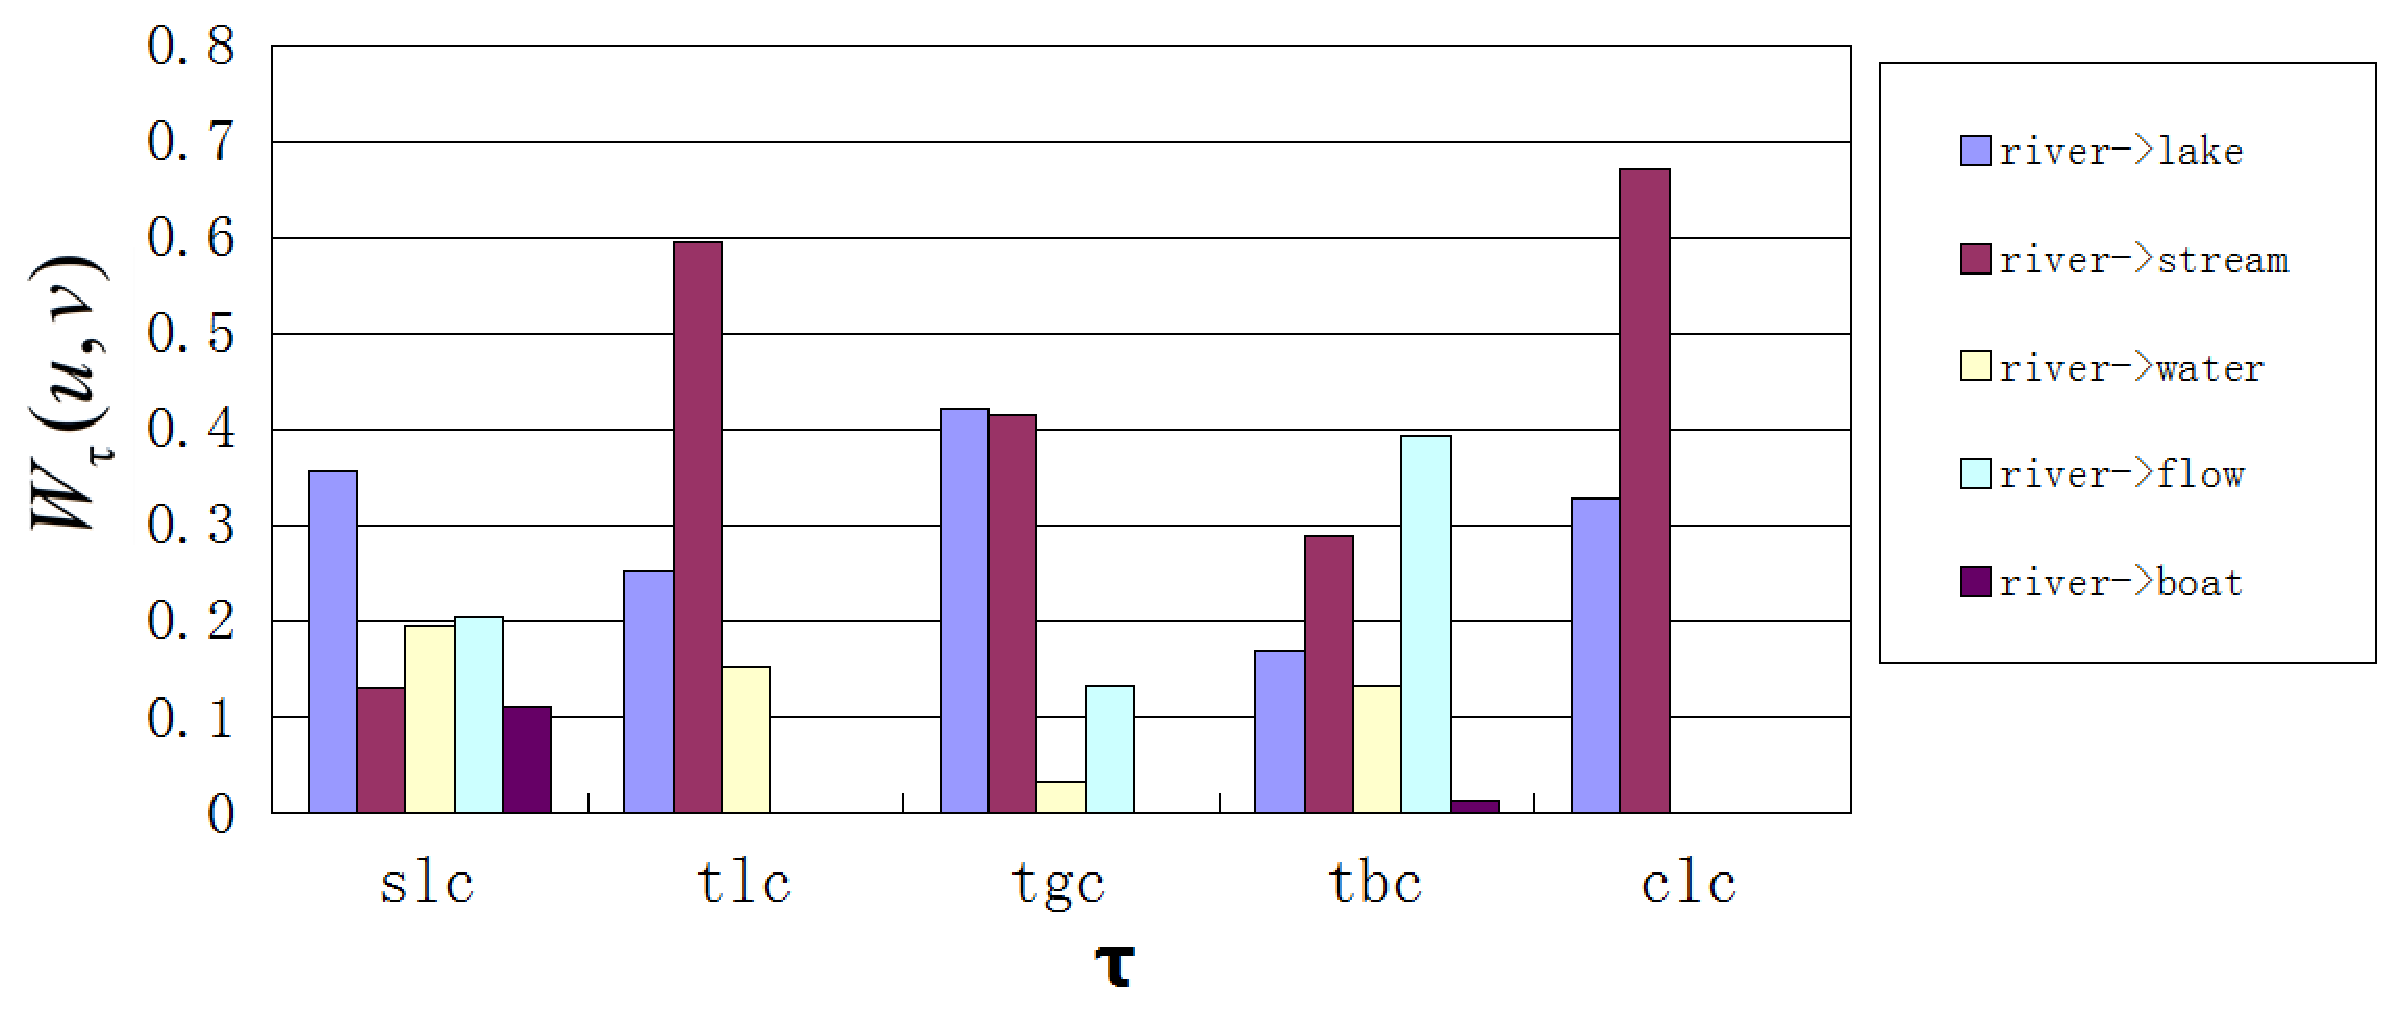
\epsfig{file=figure/distribution.eps, width=\columnwidth}
\caption{Comparison of $w_\tau(u, v)$ for different $\tau$}
\label{fig:distribution}
\end{figure}

We then integrate the five types of $w_\tau(u, v)$ into a single
strength score: $w(u, v) = \sum_{\tau}\theta_\tau w_\tau(u, v)$. 
We mimic human perception of relatedness in
determining how to aggregate co-occurrences. Specifically, we train
the weights $\theta_\tau$ through a linear regression on
the Florida Norms.

We first use the terms appearing in Florida Norms as $T_0$ to 
determine the super node set $V$. 
Then we use every cue-response pair in Florida Norms as a training
instance, with the label being the association strength computed 
form the norms.  For every training instance we
map the two terms into their corresponding super nodes $u$ and $v$, and
calculate $w_\tau(u, v)$ for every $\tau$ as its features. When
performing linear regression, we impose the constraints that
$\sum_{\tau}\theta_\tau = 1$, $0< \theta_\tau < 1$ for all $\theta_\tau$, and
that the intercept term must be equal to 0. The
parameters $\theta_\tau$ are then used to combine the different $w_\tau(u, v)$
regardless of the given $T_0$: As $\sum_{\tau}\theta_\tau = 1$ holds true, it is
easy to attest that the combined strength score $w(u, v)$ meets
the requirement of \eqref{eq:normalize}. An edge $e(u, v)$ exists
if and only if $w(u, v)>0$.

\subsection{Relatedness computation}
\label{sec:relatedness}

We now present how to leverage the constructed network for computing
relatedness between terms and between short texts.  In both algorithms,
the intention is to leverage the latent {\em bridge} 
vertices between two observed vertices to provide supportive information 
in relatedness computation.
The weight of a bridge vertex $x$, with respect to an unordered pair of 
vertices $\{u, v\}$, is defined as in \eqref{eq:bridge}.

\begin{equation}
W_{\{u,v\}}(x) = \max(w(u,x)\times w(x,v), w(v,x)\times w(x,u))
\label{eq:bridge}
\end{equation}

For term relatedness computation, we first map any given term $t$ to
its corresponding vertex $u$ in the association network. 
The relatedness between any vertex $u$ and itself is always defined to be 1:
$relate(u,u)=1$.
To compute relatedness between two vertices $u$ and $v$, 
our baseline algorithm is to add up the weights of the edges
between $u$ and $v$: 
\begin{equation}
relate(u,v)=w(u,v)+w(v,u)
\label{eq:baseline}
\end{equation} 
This algorithm captures the intuition that if $u$ associates more 
strongly to $v$ or
vice versa, $u$ and $v$ are often more related (see \tabref{tab:florida}).
As validated later in \secref{sec:eval}, despite its usefulness and 
intuitiveness in detecting related pairs, this algorithm leverages
insufficient signals from the association network and hence obtains 
sub-optimal accuracy, especially when the association network is sparse.
Thus, we propose a revised algorithm as a natural extension to the 
baseline: 
\begin{equation}
relate(u,v)=w(u,v)+w(v,u)+\sum_{x\in V}W_{\{u, v\}}(x)
\label{eq:revised}
\end{equation}
This algorithm captures the intuition that if $u$ associates more strongly to $v$, 
directly or indirectly (via some bridge vertices), or vice versa, $u$ and $v$ are often more related.

For the short text relatedness computation, 
we abstract a given text as a bag of super nodes, i.e., a vector with each
dimension being a super node and weight in that dimension being
the occurrence frequency of the terms mapping to this super node. While
cosine similarity could be directly computed to measure if two text
vectors are similar or not, it suffers from low accuracy as
semantically similar texts do not necessarily share identical or
synonymous terms with each other. 
Therefore, we expand
the original vectors before computing cosine similarity between two
vectors, by adding bridge vertices identified through our
association network as new dimensions. Algorithm \ref{algo:expand}
shows how we convert the original vector $vec_0$ to the expanded
vector $vec_+$, where $K$ is a parameter controlling the extent of 
the expansion (i.e., higher $K$ means more expanded vertices).

\begin{algorithm}[th]
\caption{Expand vector}
\label{algo:expand}
\begin{algorithmic}[1]
\Function{ExpandVector}{network $G(V, E)$, vector $vec_0$, integer $K$}
\State $vec_+ \leftarrow vec_0$
\For{$u,v \in$dimension set of $vec_0$ and $u\ne v$}
\State $V_K$ = top $K$ vertices in $V$ sorted by $W_{\{u,v\}}$
\For{$x \in V_K$}
\State $vec_+(x) \leftarrow vec_+(x) + 1$
\EndFor
\EndFor
\State \textbf{return} $vec_+$
\EndFunction
\end{algorithmic}
\end{algorithm}

\subsection{Discussion}
\label{sec:discussion}

Instead of disambiguating the term occurring in a Wikipedia page to
one of its concepts and defining each vertex to be a disambiguated
concept in the association network, we choose to define each vertex
to be a super node, comprising multiple concepts for a term.
That is because, even though it is possible to disambiguate a term
in Wikipedia pages by taking advantage of contextual information,
such a task is more difficult on the free association norms, where
virtually no context is available. Even worse, the two end-to-end
tasks (term and short text relatedness) also
inherently lack context information to perform reliable
disambiguation.

When computing the association strength between two super nodes $u$ and
$v$, the parameter $\alpha$ needs to be chosen to instantiate the
general form shown in \eqref{eq:cooccur}. One natural choice is to
set $\alpha$ to be 0, which turns the formula into conditional
probability, i.e., the probability of observing $v$, given $u$.
However, it is argued previously \cite{Wettler:1993,asso09} that 
the conditional probability measure does not take into consideration the
general frequency of the response word and therefore tends to bias
toward highly frequent words, such as function words. As a result, 
we follow \cite{Wettler:1993} to set $\alpha$ to be 0.66, 
which, according to them, perform the best in estimating word association. 

Our algorithms for relatedness computation are for showcasing the power of 
the association network, and thus many other algorithms
can be developed to  take advantage of the full potential of the association network.

\section{Experimental Results}
\label{sec:eval}

This section primarily evaluates two association networks, one
constructed only using the original free association norms (denoted
as $AN_{free}$), and the other constructed through the approach
proposed in \secref{sec:approach} (denoted as $AN_{wiki}$). The
results on $AN_{free}$ show the usefulness as well as limitations of free association
norms, while the results
on $AN_{wiki}$ validate the added benefits of Wikipedia structures 
in working around the two limitations of $AN_{free}$, leading to
better performance in semantic relatedness computation tasks.~\footnote{A demo of our system is available at
\url{http://adapt.seiee.sjtu.edu.cn/~keyang/assoc/}.}
\subsection{Data sources and statistics}
\label{sec:statistics}

The original Florida free association norms data
contains 5,019 cue words (which form the set of {\em normed words})
and a total of 72,176 cue-response pairs.
63,619 of these pairs contain responses that are also normed words.
These pairs are called {\em normed pairs} 
with known forward (cue-to-target) and backward (from target-to-cue) strengths.

Our baseline association network, $AN_{free}$, is made up of the 5019
normed words as vertices and the 63,619 normed pairs as directed edges.
Each edge carries a normalized weight $w(u, v)$, which is
proportional to $Pr(v ~|~ u)$,
Note, in $AN_{free}$, each word forms a super node by itself, as we aim to
evaluate usefulness of the original free association norms, without
depending on additional knowledge (e.g., Wikipedia) to construct super nodes.

Our proposed synthetic association network, $AN_{wiki}$, consists of 17,469
vertices (super nodes) and 107M directed edges.
This network is constructed using the 20,000 most
common English words (with stop words removed) as given $T_0$, and using
a Wikipedia dump from July, 2014.

Our test set for evaluting term relatedness is the well-known
{\em WordSimilarity-353} \cite{WS353} (a.k.a. WS-353 with 353 word pairs), 

For testing short text similarity, we use the well-known public set
{\em Li30} \cite{li06}, comprising 30 pairs of short texts. A newly constructed dataset
STSS-131 \cite{STSS131} is used to tune the parameter $K$ decribed in
Algorithm \ref{algo:expand}.


\subsection{$AN_{free}$ v.s. $AN_{wiki}$}
\label{sec:free}
To illustrate the usefulness of free association network, as well as
its limitation in semantic relatedness computation, we create WS-227,
a subset of WS-353, in which all words belong to some vertex in
$AN_{free}$.

The baseline algorithm with \eqref{eq:baseline} as its metric 
is denoted by $AN^0$, while the revised algorithm with \eqref{eq:revised} as its metric is denoted by $AN^+$.
We apply $AN^0$ and $AN^+$
using $AN_{free}$ and $AN_{wiki}$ on WS-227 and WS-353, and compare the performance measured in Spearman
correlation with two other well-known algorithms, namely
LSA \cite{LSA} and ESA \cite{ESA}, in \tabref{tab:ws227}. The result
for LSA is obtained from the widely used online
portal\footnote{http://lsa.colorado.edu/}, while the result for ESA is obtained from
ESAlib\footnote{http://ticcky.github.io/esalib/}.

We observe the following:
1) $AN_{free}^+$ performs better than LSA and ESA on WS-227,
despite its relatively small size, which suggests that free
association can be useful in computing semantic relatedness.
2) However, when tested on WS-353, due to its limited vocabulary,
$AN_{free}^+$ shows a drastic degrade in performance, which reflects
one of its primary limitations. Conversely, $AN_{wiki}$, of a larger lexical
coverage, performs consistently well on both WS-227 and WS-353.
3) Due to $AN_{free}$'s another limitation, sparseness, $AN_{free}^0$ 
exhibits sub-optimal performance on both WS-227 and WS-353; while 
$AN_{free}^+$ shows a significant improvement as the sparseness 
problem is alleviated by leveraging the latent bridge vertices. 
4) Though the best performance is obtained by $AN_{wiki}^+$, its advantage
over $AN_{wiki}^0$ is not large. We argue that it is because by 
reverse-engineering the association strength into an aggregation 
function of a vector of structured co-occurrence,
$AN_{wiki}$ alleviates sparseness by enabling to infer the edge weights missing 
in $AN_{free}$. 

\begin{table}[ht]
\centering
\caption{Spearman correlation on two WS datasets}
\begin{tabular}{lccc}
\hline
Methods & WS-227 & WS-353 \\
\hline
LSA & 0.542 & 0.579 \\
ESA & 0.727 & 0.744 \\
$AN_{free}^0$ & 0.645 & 0.476 \\
$AN_{free}^+$ & 0.752 & 0.512 \\
$AN_{wiki}^0$ & 0.758 & 0.785 \\
$AN_{wiki}^+$ & {\bf0.782} & {\bf0.813} \\
\hline
\end{tabular}
\label{tab:ws227}
\end{table}

\subsection{Prediction of free association}
\label{sec:predict}

In this experiment, we evaluate if $AN_{wiki}$ can be used to
predict free association strengths given by humans. We compute
Spearman correlation between scores predicted by a number of
competing methods \cite{asso09} and the human association strength
computed from the Kent's free association norms \shortcite{kent1910study}.
Our method is just mapping the two terms to vertex $u$ and $v$, and
assigning $w(u,v)$ as predicted association strength. 

As is shown in \tabref{tab:predict},
$AN_{wiki}$ does a reasonable job in simulating free association,
compared with other common approaches. And as a reference, the
Spearman correlation between the human labeled scores of Kent dataset and those of the Minnesota
dataset \cite{Minnesota} using the same set of cue words is 0.4,
which can be viewed as an upper bound for computer-based systems.
\begin{table}[ht]
\centering
\caption{Association Prediction}
\begin{tabular}{lcc}
\hline
Methods & Spearman  \\
\hline
Cond. Prob. & 0.31 \\
SCI & 0.34 \\
PMI & 0.28 \\
Dice/Jaccard & 0.32 \\
$AN_{wiki}$ & {\bf0.37} \\
\hline
\end{tabular}
\label{tab:predict}
\end{table}


\subsection{End-to-end tasks: term \& short text relatedness}
\label{sec:term}

\tabref{tab:ws353} compares $AN_{wiki}$ with a number of previous
approaches on the term relatedness computation using WS-353 dataset. 
Our association network achieves
state-of-the-art results on correlation with human scores.

\begin{table}[ht]
\centering
\caption{Spearman correlation on WS-353 dataset}
\begin{tabular}{lccc}
\hline
Methods & Spearman \\
\hline
Resnik \shortcite{Resnik:1995}  & 0.353 \\
LSA-Landauer \shortcite{LSA_353}  & 0.581 \\
Lin \shortcite{Lin:1998} & 0.348 \\
Roget-Jarmasz \shortcite{Roget_Jarmasz} & 0.415 \\
ESA-Gabrilovich \shortcite{ESA}  & 0.75 \\
Agirre \shortcite{Agirre:2009} & 0.78 \\
Reisinger \shortcite{reisinger2010multi} & 0.77 \\
SSA-Hassan \shortcite{SSA} & 0.629 \\
TSA-Radinsky \shortcite{TSA}  & 0.80 \\
CLEAR-Halawi \shortcite{CLEAR}  & 0.810 \\
Xu \shortcite{NET}  & 0.683 \\
$AN_{wiki}$  & {\bf0.813} \\
\hline
\end{tabular}
\label{tab:ws353}
\end{table}

\tabref{tab:li30} shows that our association network outperforms all
existing approaches by significant margins on short text similarity
task.

Recall that, Algorithm \ref{algo:expand} is parameterized by $K$
determining the extent of expansion. Our reported results use
$K=10$, empirically tuned based on STSS-131 dataset.

\begin{table}[ht]
\centering
\caption{Pearson and Spearman correlation on Li30 dataset}
\begin{tabular}{lcc}
\hline
Methods& Pearson & Spearman \\
\hline
STASIS-Li \shortcite{li06} & 0.816 & 0.813 \\
LIU \shortcite{Liu_STSS} & 0.841 & 0.854 \\
LSA-OShea \shortcite{LSA_STSS} & 0.838 & 0.871 \\
STS-Islam \shortcite{STS} & 0.853 & 0.838 \\
Omiotis-Tsatsaronis \shortcite{Omiotis} & 0.856 & 0.891 \\
WSD-STS-Ho \shortcite{SPD-STS} & 0.864 & 0.834 \\
SPD-STS-Ho \shortcite{SPD-STS} & 0.895 & 0.903 \\
SSA-Hassan \shortcite{SSA} & 0.881 & 0.878 \\
LDA-Guo \shortcite{WTMF} & 0.842 & 0.866 \\
WTMF-Guo \shortcite{WTMF} & 0.898 & 0.909 \\
WTMF+PK-Guo \shortcite{WTMF+PK} & 0.902 & -- \\
$AN_{wiki}$ & {\bf0.942} & {\bf0.940} \\
\hline
\end{tabular}
\label{tab:li30}
\end{table}

\subsection{Effects of different co-occurrences and free association training}
\label{sec:comparison1}
In this experiment, we compare an association network built from
only sentence-level co-occurrences (slc), an association network with 5 types of
co-occurrences uniformly combined (uniform), and our proposed network, which
comes with weights trained from free association norms.
\tabref{tab:comparison1} gives rise to these observations:
i) $AN_{wiki}$(uniform) outperforms $AN_{wiki}$(slc) by a large margin
on both tasks, which shows that the four additional types of co-occurrences
are useful in capturing signals not available in slc;
ii) $AN_{wiki}$ further improves the results from $AN_{wiki}$(uniform)
by a substantial margin, which shows that signals tapped from
free association norms can indeed benefit semantic relatedness computation tasks.

\begin{table}[ht]
\centering
\caption{Several variants of $AN_{wiki}$}
\begin{tabular}{lcc}
\hline
Methods & WS-353 & Li30\\
\hline
$AN_{wiki}$(slc) & 0.734 & 0.884\\
$AN_{wiki}$(uniform) & 0.766 & 0.903\\
$AN_{wiki}$ & {\bf0.813} & {\bf0.942}\\
\hline
\end{tabular}
\label{tab:comparison1}
\end{table}

\subsection{Execution time}
\label{sec:time}
Average execution time for computing the relatedness score for a pair of
terms in WS-353 is $10.3ms$, and for a pair of short texts in Li30 is $465.3ms$.
The time and space consumption can be further reduced
by filtering out edges with insignificant weights. Experiments show that
by removing up to 90\% of the edges, the accuracy in both term and short text
relatedness remains virtually constant,
and at the same time the execution time for a pair of terms and a pair 
of short texts are reduced to $1.4ms$ and $19.1ms$, respectively.

\section{Related Work}
\label{sec:related}

In this section, we introduce a number of studies
in {\em semantic relatedness computation}
and related work in {\em free association}.

Previous approaches to semantic relatedness pursue two main
directions, of using hand-crafted lexical taxonomies like
WordNet \cite{Miller1995} or Roget's Thesaurus \cite{Roget} as
semantic knowledge, or of employing probabilistic approaches to
decode semantics based on large corpora.

The first approach of using hand-crafted resources proposes
knowledge-based measures that tap into the properties of their underlying
structure to compute semantic relatedness
 \cite{Roget,Lin:1998,leacock1998,Hirst:1998,Jiang:1997,Resnik:1995,wu1994verbs}.
Though showing potential in such tasks like term relatedness
computation, this approach requires to construct manually curated lexical
resources and thus cannot easily scale to larger lexical coverage or
to a new language.

On the other hand, the second approach of using corpus-based
measures, instead of relying on human-organized knowledge, utilize
the contextual information and patterns observed in large corpus to
construct semantic profiles for words. Latent Semantic Analysis
(LSA) \cite{LSA} was an original approach to leverage word
co-occurrences from a large corpus of text, and ``learns''
its representation by applying Singular Value Decomposition to
the words-by-documents co-occurrence matrix. Explicit Semantic Analysis
(ESA) \cite{ESA} as well as Salient Semantic Analysis (SSA) \cite{SSA}
were proposed to incorporate large amounts of human
knowledge such as Wikipedia into word
relatedness computation. They both represent a word as a concept
vector, where each dimension corresponds to a Wikipedia concept.
Later, Temporal Semantic Analysis (TSA) \cite{TSA} considered that
words have different meanings over time and extended the concept
vector with a temporal dimension.
To bridge the corpus-based measures with
knowledge-based measures, Constrained LEArning of Relatedness (CLEAR) \cite{CLEAR}
was proposed to learn word
relatedness based on word occurrence statistics from large corpora
while constraining the learning process by incorporating knowledge
from WordNet.  Some recent works like \cite{mikolov} used machine learning techniques
to compute continuous vector representations of words from large datasets
, shown to perform better than LSA for preserving linear regularities among words.

Some models aim particularly at solving the similarity problem
between two sentences, or two short
texts \cite{WTMF,WTMF+PK,SPD-STS,LSA_STSS}. WSD-Based Sentence
Similarity \cite{SPD-STS} was proposed to compute the similarity
between two sentences based on a comparison of their actual meanings
by integrating word sense disambiguation. WTMF \cite{WTMF} was
proposed to model the missing words in the sentences as a typically
overlooked feature to address the sparseness problem for the short
text similarity task.

All the existing semantic relatedness models mentioned above, though
leveraging some useful signals from hand-crafted lexical taxonomies
or large corpus text, fail to actively take advantage of the human
perception signal in semantic relatedness computation. Our approach,
by effectively bridging this gap using signals in the well-studied
psychological process of free association, outperforms
state-of-the-art models in both word and short text relatedness
tasks.

Free association is a task requiring human participants to produce the
easily associated word for the given cue word, to tap into human perception acquired through
world experience \cite{Nelson:2004}.
Mining the signals contained in this cognitive process
is made possible by several collections of free association norms
 \cite{Nelson:2004,kent1910study,Minnesota,kiss1973associative},
which are typically collected by researchers in phychology and
cognitive science. As the Florida Norms is the
largest collection available, and also the most recent in time,
we choose to use it as our primary source of human perception
to be combined with signals from Wikipedia.

\section{Conclusion}
\label{sec:conclude}

We synthetically
build an association network, by aggregating Wikipedia
signals, using free association as a training data. 
Our evaluation results
validated that our proposed framework reaches state-of-the-art
in a standard benchmark for term relatedness computation and
outperforms all other state-of-the-arts for short text similarity
computation by a significant margin.

\section*{Acknowledgement}
Kenny Q. Zhu, the contact author, was supported by
NSFC grant 61373031 and NSFC-NRF Joint Research Program.
Seung-won Hwang was supported  under the framework of international 
cooperation program managed by NRF of 
Korea (2014K2A2A2000519). This work received contributions from
Kailang Jiang and Jinyi Lu.

\bibliographystyle{aaai}
{\small
\bibliography{./asso}}
\end{document}
